%\chapter{Vorlesung}
\section{Definition: Sperrfluss}
\[ G=(V,E)~~g:E\rightarrow\mathbb{R}^+\text{ ein Fluss} \]
Auf jedem $s-t$-Pfad gibt es eine saturierte Kante $(u,v)\in E$, d.h. $g(u,v)=c(u,v)$
\paragraph{Achtung}
Wir betrachten hierbei \underline{nicht} die Kantenmenge $E_f$ des Restnetzwerkes.\\
Es gilt: $~~\delta_{f'}(s,v)\geq \delta_f(s,v)$, wobei $f'$ aus $f$ durch eine Flusserhöhung hervorgegangen ist.\\
Für den Dinic-Algorihtmus gilt darüber hinaus, dass $\delta_{f'}(s,t) \geq \delta_f(s,t)+1$ wobei $f'$ aus $f$ durch eine Flussverbesserung mittels eines Sperrflusses $g$ hervorgegangen ist.
\pagebreak
\paragraph{Beweisidee}
%Grafik 2 und 3
\begin{figure}[h]
\centering
\begin{subfigure}[H]{0.4\linewidth}
	\centering
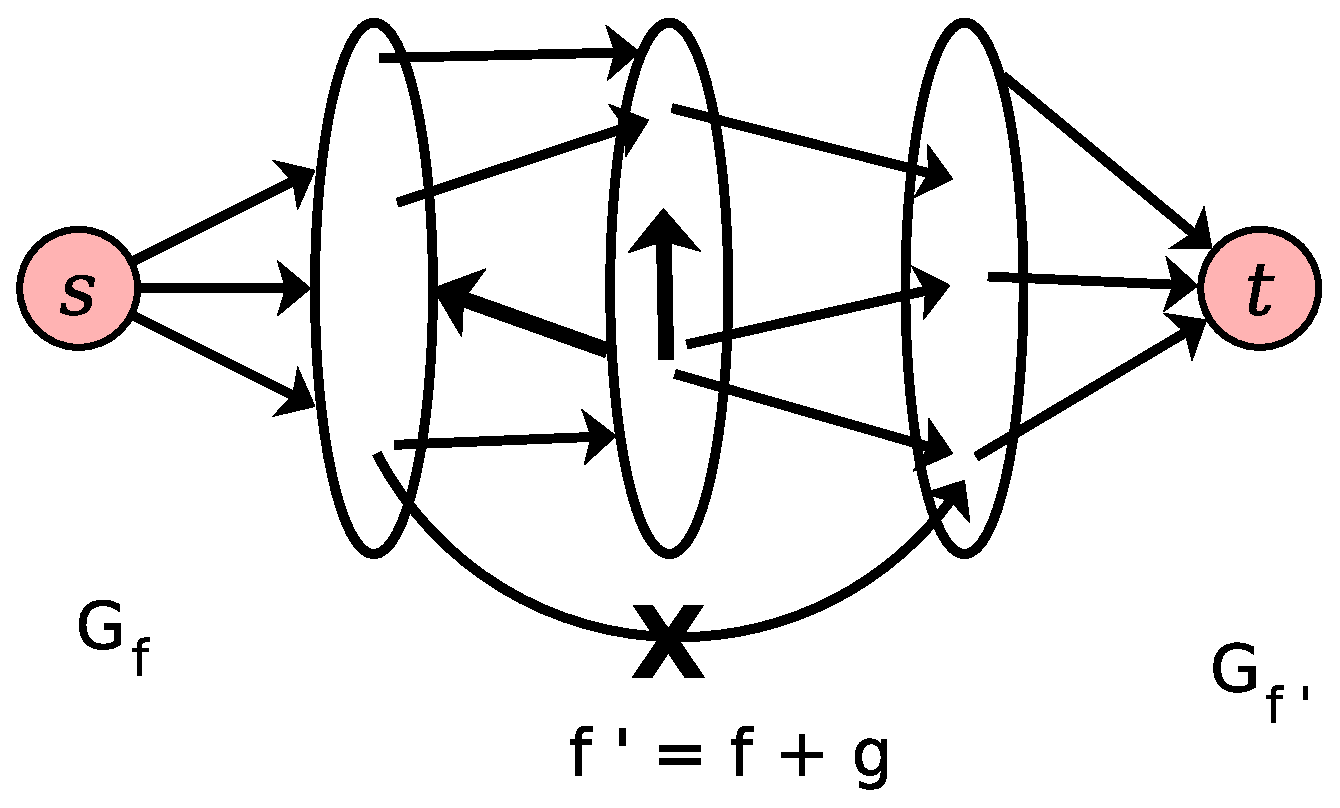
\includegraphics[width=\linewidth]{27/Grafik/Diagramm2}
\caption{$g$ Sperrfluss}
\label{fig:Diagramm2}
\end{subfigure}
\hspace*{60pt}
\begin{subfigure}[H]{0.4\linewidth}
	\centering
	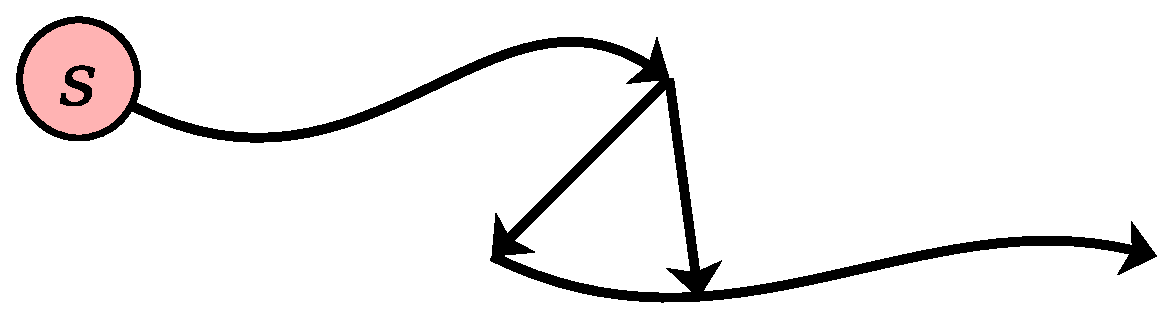
\includegraphics[width=\linewidth]{27/Grafik/Diagramm3}
	\caption{}
	\label{fig:Diagramm3}
\end{subfigure}
\end{figure}
\paragraph{Konsequenz}
Im Dinic-Algorithmus genügt es, $|V|$ Sperrfluss-Berechnungen durchzuführen.
\paragraph{Ziel}Sperrfluss in Zeit $\mathcal{O}(|V|\cdot|E|)$ berechnen.
\begin{align*}
\text{Gesamtlaufzeit }&\text{Dinic }&\mathcal{O}(|V|^2\cdot|E|)\\
\text{vs. }&\text{Edmonds-Karp }&\mathcal{O}(|V|\cdot|E|^2)\\
&\text{(Sleator \& Tarjan :}& \mathcal{O}(|V|\cdot|E|\cdot\log|V|))
\end{align*}
\subsection{Pseudo-Code}
\begin{lstlisting}[style=pseudo]
H = $G^L_f$;
stack P;
P.push(s);
g = 0;
while(true) {
	u = P.top();
	if ($\exists$ (u, v) $\in$ H) {
		P.push(v);
		if (v $\neq$ t) continue;
		//v = 7, d.h. flussverbessernder s-t-Pfad gefunden
		$c_{min}$ = $\underset{\text{(u,v)}\in P}{\min} \{ \text{c}_f\text{(u, v)-g(u, v)} \}$
		forall $(u,v)\in P$ {
			g(u, v) = g(u, v)+c$_{min}$;
			if (g(u, v) == c$_f$(u, v))
				lösche (u, v) $\in$ H;
		}
		P.clear();
		P.push(s);
		continue;
	} //end if
	//Sackgasse
	lösche alle zu u inzidenten Kanten aus H;
	P.pop();
	if (u == s)
		break;
} //end while
\end{lstlisting}
\subsection{Begründung zur Laufzeit}
Jeder $s-t$-Pfad wird in Zeit $\mathcal{O}(|V|)$ gefunden. Danach wird mindestens eine Kante aus $H$ entfernt, weil sie saturiert wird. Jede kante kann höchstens einmal als Sackgasse betreten werden, weil sie anschließend gelöscht wird.
\section{Maxmimum Matching als Flussproblem}
\begin{figure}[H]
	\begin{subfigure}[H]{0.4\linewidth}
		\centering
		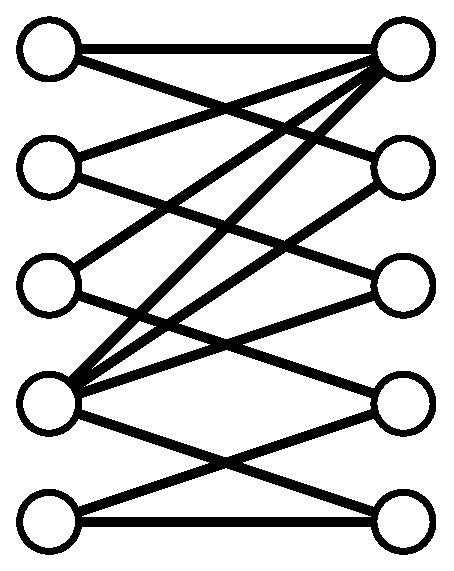
\includegraphics[width=0.5\linewidth]{27/Grafik/Diagramm4}
		\caption{Matchingproblem}
		\label{fig:Diagramm4}
	\end{subfigure}
	\begin{subfigure}[H]{0.4\linewidth}
		\centering
		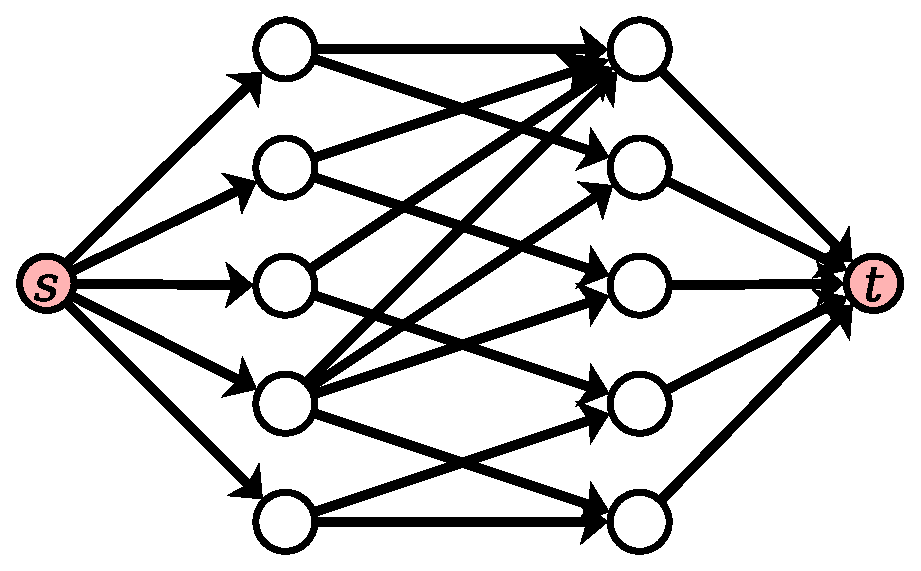
\includegraphics[width=\linewidth]{27/Grafik/Diagramm5}
		\caption{Flussproblem (Kantengewichte sind 1)}
		\label{fig:Diagramm5}
	\end{subfigure}
\end{figure}
\[ E \supseteq M^* = \{ (u,v)\in E \cap V_1\times V_2 ~|~ f(u,v) = 1 \} \]
\begin{align*}
\text{F.F.-Laufzeit }~~ &\mathcal{O}(|f^*|\cdot|E|)\\
&=\mathcal{O}(|V|\cdot|E|)
\end{align*}

$|f|$ ist ganzzahlig $=$ Kardinalität des maximum Matchings $|M^*|$
\subsection[Flussnetzwerke mit Einheitskapazität]{Flussnetzwerke mit Einheitskapazität (unit capacity network flow)}
\[ G=(V,E)~~c:E\rightarrow\{0,1\} \]
Sperrfluss-Berechnung läuft in $\mathcal{O}(|E|)$, weil immer alle Kanten auf den flussverbessernden $s-t$-Pfaden gelöscht werden können.
\paragraph{Dinic:} $\mathcal{O}(|V|\cdot|E|)$
\subsubsection{Satz}
Mit Hilfe des Dinic-Algorithmus lässt sich ein Flussproblem mit Einheitskapazität in Zeit 
\[ \mathcal{O}\left( \min\left( |E|^\frac{1}{2},|V|^\frac{2}{3} \right) \right) \]
lösen.
\subsubsection{Beweis}
\paragraph{1. Fall}
Zeige, dass $2\cdot\sqrt{|E|}$ viele Sperrfluss-Berechnungen genügen.
\subparagraph{1. Phase} Zuerst $\sqrt{|E|}$ Sperrfluss-Berechnungen. $\Rightarrow$ Fluss $f$ 
\[ \Rightarrow\delta_f(s,t)\geq \sqrt{|E|} \]
\begin{figure}[h]
	\centering
	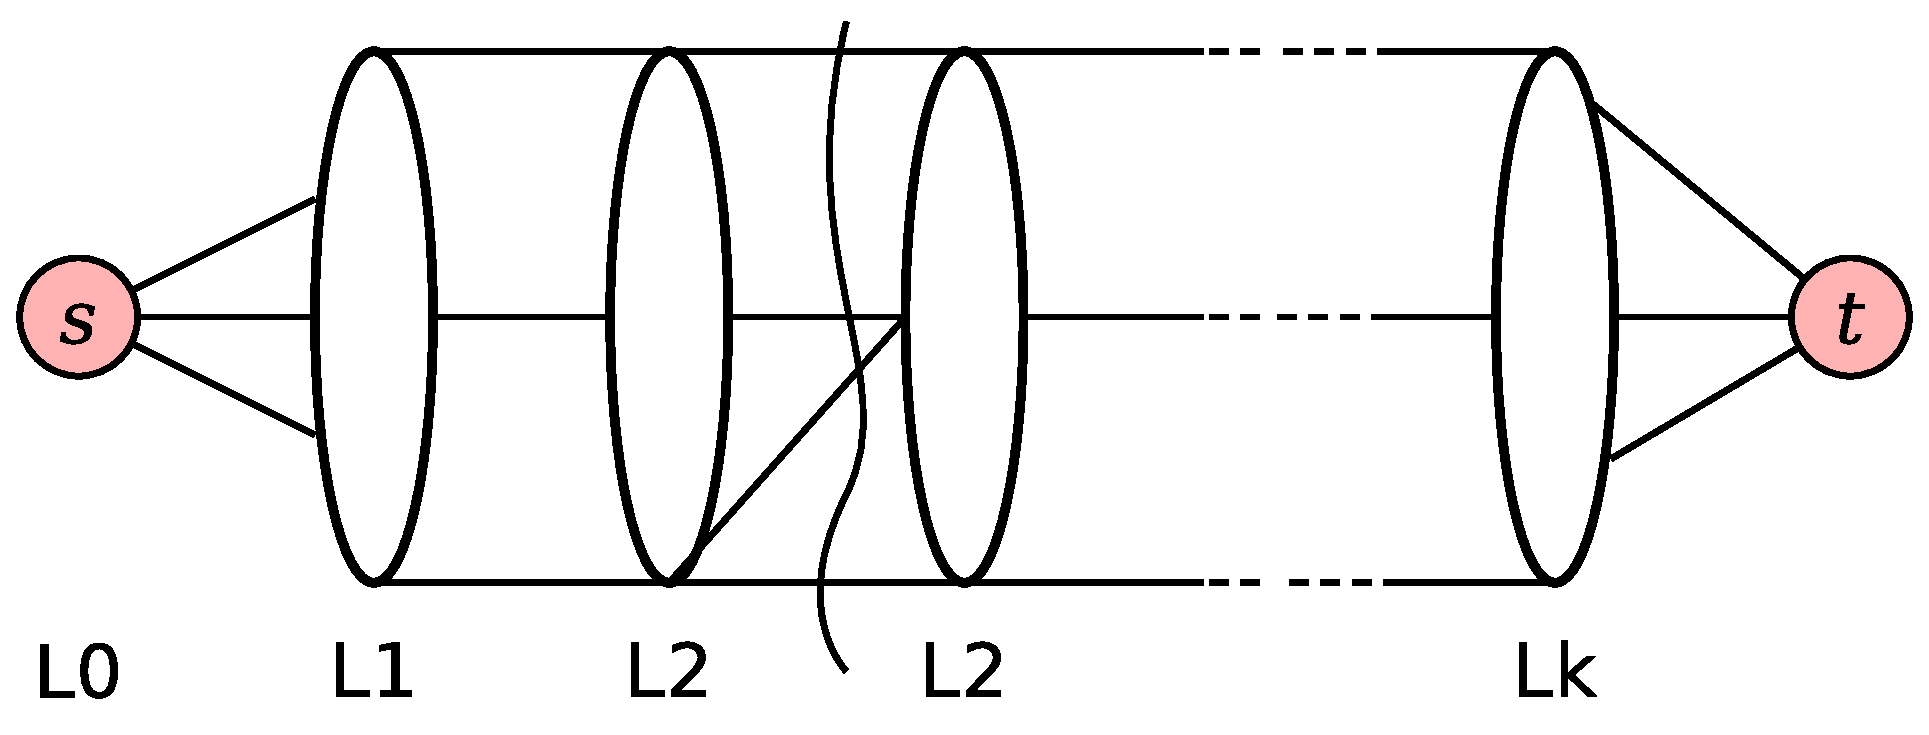
\includegraphics[width=0.7\linewidth]{27/Grafik/Diagramm6}
	\caption{$k\geq \sqrt{|E|}$}
	\label{fig:Diagramm6}
\end{figure}
$\Rightarrow$ Schnitt zwischen zwei Levels $L_i$ und $L_{i+1}$ mit weniger als $\sqrt{|E|}$ Kanten.\\
$|f^*| \leq |f| +\sqrt{|E|}$, weil über diesen Schnitt zusätzlich zu $f$ noch ein Fluss der Größe $\sqrt{|E|}$ möglich ist.\\
\subparagraph{$\Rightarrow$ 2. Phase:}
Um von $f$ zu $f^*$ zu kommen, reichen weitere $\sqrt{|E|}$ viele Sperrfluss-Berechnungen aus.